% --- Aufgabenblatt: Vorrangregeln beim Rechnen ---

\section*{Vorrangregeln beim Rechnen}

\textbf{Merke:} Punktrechnung (\textbf{Mal} und \textbf{Geteilt}) geht vor Strichrechnung (\textbf{Plus} und \textbf{Minus}). Klammern haben immer Vorrang!

\begin{center}
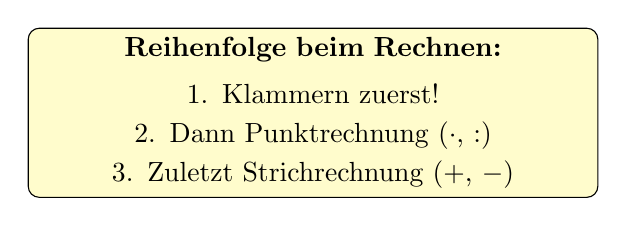
\begin{tikzpicture}[scale=1]
  \node[draw, fill=yellow!20, rounded corners, text width=7cm, align=center] at (0,0) {
    \textbf{Reihenfolge beim Rechnen:} \\[0.5em]
    1. Klammern zuerst! \\[0.2em]
    2. Dann Punktrechnung ($\cdot$, $:$) \\[0.2em]
    3. Zuletzt Strichrechnung ($+$, $-$)
  };
\end{tikzpicture}
\end{center}

\subsection*{1. Rechne aus (ohne Klammern)}
\begin{multicols}{2}
\begin{enumerate}[a)]
    \item $3 + 4 \cdot 2$
    \item $12 - 6 : 2$
    \item $5 \cdot 2 + 7$
    \item $18 : 3 - 2$
    \item $6 + 8 \cdot 2$
    \item $20 - 4 \cdot 3$
    \item $7 + 12 : 4$
    \item $9 \cdot 2 - 5$
\end{enumerate}
\end{multicols}

\subsection*{2. Rechne aus (mit Klammern)}
\begin{multicols}{2}
\begin{enumerate}[a)]
    \item $(3 + 4) \cdot 2$
    \item $12 - (6 : 2)$
    \item $5 \cdot (2 + 7)$
    \item $(18 : 3) - 2$
    \item $(6 + 8) \cdot 2$
    \item $20 - (4 \cdot 3)$
    \item $7 + (12 : 4)$
    \item $(9 \cdot 2) - 5$
\end{enumerate}
\end{multicols}

\subsection*{3. Setze Klammern, so dass das Ergebnis stimmt}
\begin{enumerate}[a)]
    \item $2 + 3 \cdot 4 = 20$
    \item $18 - 6 : 2 = 6$
    \item $5 \cdot 2 + 3 = 16$
    \item $12 - 2 \cdot 5 = 10$
    \item $8 + 4 \cdot 2 = 24$
    \item $16 - 8 : 2 = 4$
\end{enumerate}

\subsection*{4. Textaufgaben}
\begin{enumerate}[a)]
    \item Ein Kinoticket kostet 8 €. Wie viel kosten 3 Tickets und 2 Getränke à 3 € zusammen?
    \item In einer Klasse sind 5 Gruppen mit je 4 Schülern. Jeder Schüler bekommt 2 Hefte. Wie viele Hefte werden insgesamt benötigt?
    \item Ein Rechteck hat die Seitenlängen 6 cm und 4 cm. Berechne den Umfang und den Flächeninhalt.
    \item Ein Bus fährt 120 km in 2 Stunden. Wie viele Kilometer fährt er in 5 Stunden?
\end{enumerate}

\subsection*{5. Knobelaufgabe}
\textbf{Setze Klammern:} $8 - 2 \cdot 3 + 4 = 10$\\
\textbf{Tipp:} Probiere verschiedene Klammer-Setzungen aus!

\vspace{1em}
\textbf{Extra:} Erfinde selbst eine Aufgabe, bei der die Klammern das Ergebnis verändern!